\documentclass[../main.tex]{subfiles}
\begin{document}

\subsection{Reeks A}

\subsubsection{Vaardigheden}
\begin{question}Met de opkomst van digitale rekentoestellen hebben fervente aanhangers van de oudere rekenhulpmiddelen beweerd dat een aantal rekenvaardigheden verloren zouden gaan, o.a. het schatten van de grootte van het resultaat. Denk je dat de actuele ontwikkelingen op het gebied van ICT ook een aantal vaardigheden doen verloren gaan?
\end{question}

\begin{solution}
	Hieronder een aantal vaardigheden die verloren kunnen gaan door de huidigen ontwikkelingen op het gebied van ICT:
	\begin{enumerate}
		\item \textbf{Geheugen:} We hebben tegenwoordig altijd computers binnen handbereik (Smartphone). Informatie die men vroeger zou moeten noteren en eventueel memoriseren kunnen nu snel opgezocht worden. Vroeger was het niet ongewoon
		om telefoonnummers van buiten te kennen. Nu hebben we allen een telefoonboek in onze zak.
		\item \textbf{Kennis:} Dankzij de computers is alle informatie vrijwel direct vindbaar. Mensen doen dus minder opzoekingswerk in bijvoorbeeld bibliotheken. Hierbij wordt ook de drang om bekomen informatie te memoriseren minder groot.
		Terwijl het vroeger nogal wat moeite kostte om informatie op te zoeken, gebeurt dit tegenwoordig vrijwel moeiteloos. Bovendien moedigt dit oppervlakkige kennis aan van materie, door de overvloed aan beschikbare informatie die tevens niet altijd correct is, wordt er minder grondig gelezen.
		\item \textbf{Afspraken maken:} Een afspraak afzeggen of last minute verplaatsen ging vroeger moeilijker dan vandaag (dankzij Telecom). Mensen hielden zich dan ook meer aan afspraken in plaats van last minute af te zeggen of wijzigingen aan te brengen.
		\item \textbf{Navigatie:} De opkomst van de GPS heeft het gebruik van de fysieke kaart grotendeels vervangen. Vroeger vereiste navigatie ori\"entatievermogen.
		\item \textbf{Sociaal:} We kunnen alles ogenblikkelijk delen met iedereen die we willen via sms, sociale netwerken of email. Hierdoor wordt er misschien minder echt gepraat dan vroeger, aangezien je vaak alles al verteld hebt via voorgaande media!

	\end{enumerate}
\end{solution}

\subsubsection{Basissen Getallensystemen}
\begin{question}
Welke basissen van getallensystemen zijn er in de loop van de geschiedenis gebruikt en waar vinden we die nu nog terug?
\end{question}

\begin{solution}
	\begin{description}
			\item[Basis 60] Basis 60 vinden we terug in onze indeling van tijd. 1 uur is namelijk 60 minuten, een minuut is 60 seconden. Ook het gebruik van graden in de meetkunde verwijst naar een basis van 60. Babylonische wiskundigen gebruikten in 1750 voor Chr. het sexagesimaal positiestelsel met basis 60. Deze notatie was al floating point. Hierbij kunnen de vingerkootjes gebruikt worden om tot 12 te tellen, terwijl het andere hand kan gebruikt worden om veelvouden bij te houden. Waardoor er ook op de handen geteld kan worden tot 60.
			\item[Basis 20] In het pre-columbiaanse Amarika vinden we getallen notaties terug bij de Maya's die gebruik maken van basis 20. Ook de Franse woorden voor getallenreeksen duiden op een basis 20.
			(quatre-vingt). Bovendien werd tot enkele decennia geleden de Britse pond verdeelt in 20 shilling en elke shilling in 12 pence (basis 12).
			\item[Basis 10] Basis 10 komt ongetwijfeld van het tellen op de 10 vingers van de beide handen. In Babyloni\"e rond 1750 voor Chr. werden er tijdens handelsbetrekkingen getallen genoteerd per groeperingen per 10, per 100 enzovoort. Zij maakten dus eigenlijk gebruik van basis 10. De getallennotatie in het decimale positiestelsel die we nu kennen (voor gehele getallen) is ontstaan in India, rond 500-600 na Christus. De eerste tekenen van dit decimale positiestelsel werd teruggevonden in sterrenkundige berekeningen. Het stels is ontstaan uit een ouder Indiaas getallenstelsel met voorlopers van de symbolen voor 1 - 9.
			\item[basis 12] In vele westerse talen hebben de getallen van 1 tot en met 12 een eigen naam (bv. dozijn). Dit wijst erop dat 12 ook mogelijk ooit als basis werd gebruikt. Bovendien kan voor basis 12 geteld worden op de vingerkootjes, wat ook op de origine van deze basis kan wijzen.
			\item[Basis 2] Basis 2 wordt gebruikt in elektrische schakelingen en computers.
	\end{description}
\end{solution}

\subsubsection{Cijfer Nul}
\begin{question}
Waarom is nul belangrijk? Ken je de vermoedelijke oorsprong?
\end{question}

\begin{solution}
Rond 1750 voor Chr. gebruikten Babylonische wiskundigen een symbool voor 0 als plaatshouder, maar het werd nog niet als getal gebruikt en ook nooit achteraan of vooraan een getal geschreven. Ook werd er in het Bakshali manuscript(2de - 3de eeuw na Chr.)  al een symbool voor nul gebruikt. Sommige onderzoekers vermoeden dat het gebruik  van de nul in combinatie met eenheden een Indiase ontdekking is, die te maken heeft met de structuur van de taal, het Sanskriet. Anderen vermoeden dat ze inspiratie putten uit het Babylonis sexagesimaal positiestelsel dat met de Babylonische/Griekse sterrenkunde mee naar India is gekomen. Brahmagupta (598-670 n.Chr.) beschreef het gebruik van de nul als getal en bewerkingen met het getal nul. De Indiase getallennotatie is via de Arabische wereld naar Europa gekomen. Er was sterke interesse in Sterrenkunde en daarbij werden indiase methoden gebruikt.In 1202 publiceerde Leonardo Van Pisa (Fibonacci) ``Liber Abaci'' waarin het gebruik van arabische cijfers werd beschreven, inclusief nul. Hiermee werd het ge\"introduceerd in Europa.

Dankzij het gebruik van de nul, kunnen grote getallen gemakkelijker worden voorgesteld. In plaats van telkens een symbool te moeten verzinnen voor grote getallen, geven eenheden met daarachter nullen de grootte van een getal aan.



\end{solution}

\subsubsection{Rekenhulpmiddelen}
\begin{question}
Welke rekenhulpmiddelen heb je zelf gebruikt? Welke ken je? Welke zijn er in onbruik geraakt en waarom?
\end{question}

\begin{solution}
Hieronder is een opsomming van rekenhulpmiddelen:
	\begin{description}
		\item[Tabellen] Bij de Babylonie\"ers werden er al tabellen teruggevonden met kwadraten, derde machten en inversen. Meer recent werden tabellen ook gebruikt om bijvoorbeeld de waarden van sinus, cosinus of logaritmes op te zoeken.
		Zelf hebben we nog gebruik gemaakt van tabellen om de kansen van normaal- of andere verdelingen op te zoeken. Maar vele zijn in ongebruik geraakt door de opkomst van het moderne rekentoestel, waarmee vele waardes kunnen worden opgevraagd die we normaal uit een tabel zouden halen.
		\item[Quipu] De Inca's stelden getallen voor en bewaarde ze met behulp van knoopjes in touwen.
		\item[Kerfstok] De inkervingen hierop stellen getallen voor. Met de opkomst van systematische notatie van getallen wordt dit niet meer gebruikt.
		\item[Vingers] Tellen op de vingers kent iedereen, het is een handige manier om te tellen met basis 10 of basis 12, 60.
		\item[Abacus, telraam, rekenbord] Aantekeningen kunnen gekrast worden in zand of stof, Er zijn ook rekenborden met lijntjes en steentjes(of staafjes en kralen). Werd vooral gebruikt omdat schrijven niet verspreid was.
		\item[Rekenlineaal] Dit is een liniaal met Logaritmische afstanden. Een vermenigvuldiging en deling worden met logaritmes respectievelijk een optelling en aftrekking. Men kan dan twee logaritmische afstanden optellen/aftrekken op de liniaal om gemakkelijk het resultaat af te lezen. Een huidig zaakrekentoestel heeft het gebruik van de rekenliniaal vervangen.
		\item[Mechanisch rekenmachine] Na de middeleeuwen werd er verschillende keren getracht om een mechanisch rekentoestel te ontwikkelen, zo ontwikkelde in 1623 Wilhemm Schickard een rekenklok om aftrekken, vermenigvuldigen en optellen eenvoudiger te maken. Blaise Pascal ontwikkelde in 1642 een telmachine met radaren (Pascaline) welke kon optellen en aftrekken . In 1666 maakte Samuel Morlan een machine waarmee vermenigvuldigd kon worden. In 1694 ontwierp Gottfried Leibniz een rekentoestel waarme optellen, aftrekken, deling, vermenigvuldiging machten en vierkantswortels konden worden berekend. Deze modellen oogstten echter nooit succes (werkkracht was goedkoop en het toestel was duur). Charles Xavier de Colmar maakte patenteerde in 1820 het eerste commercieel succesvol mechanisch rekentoestel. Hierna kwamen nog succesvolle modellen. Deze werden later echter ook vervangen door elektronische rekenapparatuur.
		\item[Computers]

	\end{description}
\end{solution}
\subsubsection{Figuren: Hollerith's Machine en van Abacus naar cijferrekenen}

\begin{figure}[ht!]
	\begin{center}
		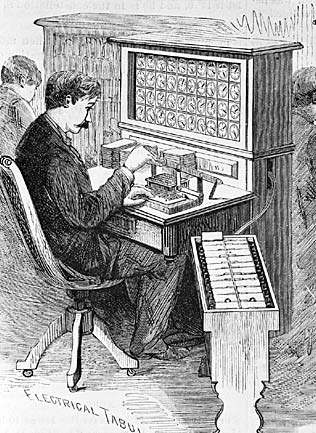
\includegraphics[scale=0.5]{ponskaarthollerith}
		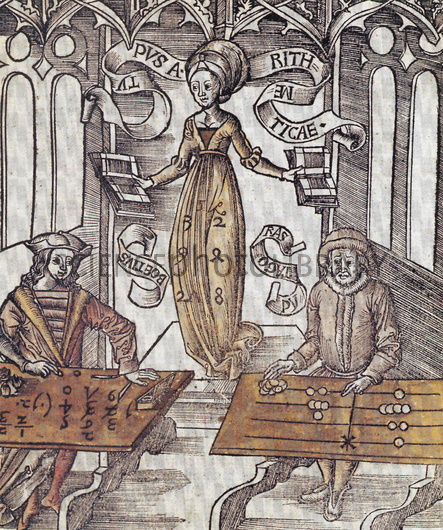
\includegraphics[scale=0.41]{algorithms}
	\end{center}
	\caption{Figuren bij vraag 5}
	\label{fig:vraag5}
\end{figure}

\begin{question}
Kan je de de figuren op Figuur \ref{fig:vraag5} thuisbrengen? Vertel wat je ervan weet.
\end{question}
\begin{description}
	\item[Linkse Figuur] De linkse Figuur is van Herman Hollerith en een van zijn Hollerith machines die tegen het einde van de negentiende eeuw in de VS gebruikt werden om volkstellingen te doen. De tellingen gingen hierdoor aanzienlijk sneller.
	 Deze machine gebruikte ponskaarten. Ze verwerkten grote hoeveelheden gegevens, voor uitvoeren van berekeningen waren ze niet geschikt.
	\item[Rechse Figuur] De rechterpersoon op deze figuur rekent met een Abacus. terwijl de linkerpersoon aan cijfer rekenen doet. Deze afbeelding duidt op de overgang naar het cijferrekenen in Europa. Deze overgan gebeurde tussen 1000 - 1200. Pater Gebert d'Aurillac (945 -1003, paus Sylvester II), bestuurde het gebruik van Arabische cijfers. Later schreef Leonardo van Pisa (Fibonnaci) in 1202 het werk Liber Abaci. Hierin wordt rekenen met arabische cijfers (inclusief nul) uitgelegd. Het tekenende dus de Europese overgang naar het rekenen met Arabische cijfers.
\end{description}


\end{document}